\documentclass[text.tex]{subfiles}

\begin{document}

\begin{figure}[h]
\centering
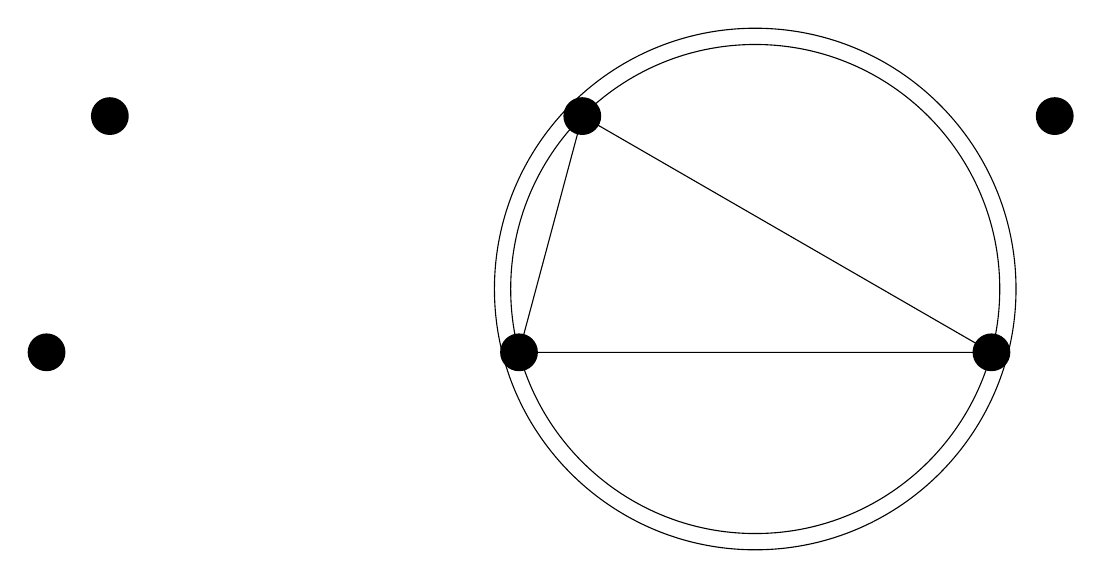
\begin{tikzpicture}[scale=6]

% nodes
\draw [-] (0,0)  -- (-1,0) -- (-0.86602540378,0.5) -- cycle;
\fill (0,0) circle (0.04);
\fill (-1,0) circle (0.04);
\fill (-0.86602540378,0.5) circle (0.04);
\fill (-2,0) circle (0.04);
\fill (-1.86602540378,0.5) circle (0.04);

\fill (1-0.86602540378,0.5) circle (0.04);

\draw (-0.5,0.13397) circle (0.5176);
\draw (-0.5,0.13397) circle (0.552);


\end{tikzpicture}
\caption{Section of the artificial quasicrystal with the circumcircle and a circle of the estimated radius.}
\label{fig:coveringRadius}
\end{figure}



\section{Estimate of covering radius}

For further analysis covering radius of the quasicrystal must be evaluated. 
Precise value is however not necessary, upper bound estimate is sufficient. 
Estimate of the covering radius is used to limit the amount of the points of the quasicrystal needed to be included in the creation of a voronoi polygon, as in Theorem \ref{the:radiusLimit}.

As a reminder, here is the definition of the covering radius $R_c$, as is in Definition \ref{def:delone}.

$$R_c = \inf\{R>0\,|\, z\in\mathbb{R}^n \exists x\in P: \|z-x\|\leq R\}$$

The estimate is derived from an artificial quasicrystal with only the largest distances between points (largest for the given window). Such quasicrystal has, for given window, certainly larger covering radius than any other. Since all such artificial quasicrystals are different only in scale and translation, the estimate is derived form a "normalized" one (a point in the origin and a unitized distance between points).

The estimate is then evaluated as the radius of a circumscribed circle or the circumradius $R$ of a triangle with vertices $(0,0)$, $(-1,0)$ and $\left(\frac{2-\beta}{2},\frac{1}{2}\right)$, as in Figure DOPLNIT. 

$$R_c \leq R = \frac{a}{2sin(\alpha)} = \frac{1}{2\left(\frac{1+\sqrt{3}}{2\sqrt{2}}\right)} = \frac{\sqrt{2}(\sqrt{3}-1)}{2}$$

Since the estimate is used in comparison with coordinates of points of the quasicrystal, it is advantageous if it is also from $\ring$. For that the estimate $1.414 \doteq \sqrt{2} <32\beta-118 \doteq 1.426$ is used.

$$\frac{\sqrt{2}(\sqrt{3}-1)}{2} < \frac{(32\beta-118)(\beta-3)}{2} = 161-43\beta \doteq 0.522$$







\begin{remark}
There is an easier way that removes the need for such deriving. Simply estimate the covering radius with the largest distance itself. That is at first sufficient, but computational complexity of quasicrystals with a general window forced us to use all optimizations available.
\end{remark}
\end{document}
